\subsection*{Экспериментальная установка}

Схкма установки, используемой в работе, показана на рис. \ref{fig:exp1}. Свинцовый коллиматор выделяет узкий, почти параллельный пучок $\gamma$-квантов, проходящий через набор поглотителей П и регистрируемый сцинтиляционным счетчиком. Сигналы от счётчика усиливаются и регистрируются пересчетным прибором ПП. Высоковольтный выпрямитель обеспечивает питание сцинтиляционного счетчика.
% см. приложение II

\begin{figure}[h]
    \centering
    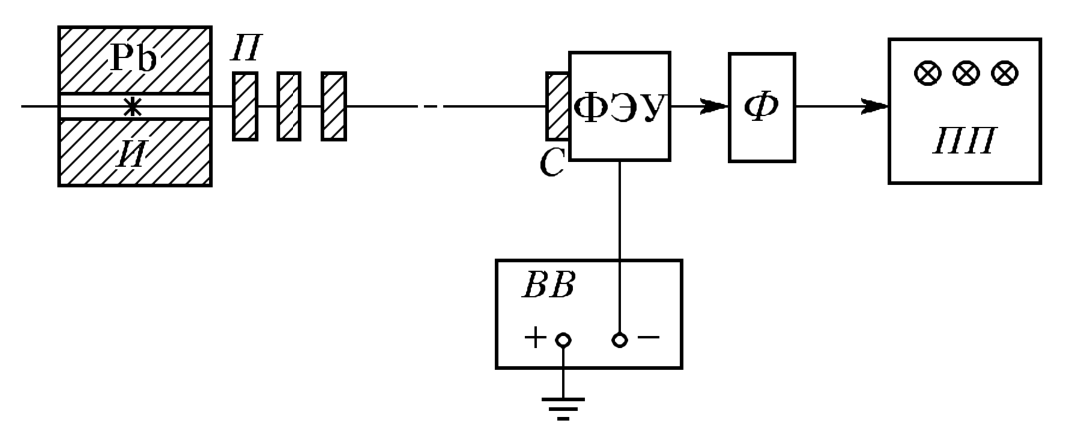
\includegraphics[width=0.5\textwidth]{figures/exp_1.png}
    \caption{Блок-схема установки. И -- источник $\gamma$-лучей, Pb -- свинцовый контейнер с колиматорным каналом, П -- набор поглотителей, С -- сцинтиллятор, Ф -- формирователь-выпрямитель.}
    \label{fig:exp1}
\end{figure}

